\chapter{}
 Morrison et al.\cite{populationDiversity} described the pair-wise Hamming distance as one of the most commonly used measures of distance in genotypic space, and is what will be used here to calculate a populations diversity as one scalar metric. In implementation, this algorithm\ref{eq:Hamming} is counting the number of genomes in all pairs of genotypes which is not identical. Another description is the edit distance between two binary genomes. 


where y is a genotype, P is the population size and L is the number of genomes in a genotype.

A problem with using a pairwise Hamming distance is that the number of computations is quadratic with the size of P. Meaning the computational time is quite long, but since this metric is only to be calculated once when experimentation is completed, the restriction this puts on the experiment is negligible. However, a suggested alternate way of calculating population diversity on the basis of edit distance is by calculating the mean edit distance from every genotype to a \textit{centroid} genotype where the centroid is the average genotype in a population, and its i-th element can be given as  
\begin{equation}
    \label{eq:centroid}
    \varphi_{i}=\tfrac{1}{P}\sum_{j=1}^{P}y_{ji}
\end{equation}
Using this vector that can be calculated linearly with respect to P, a diversity metric \(\Delta\) can be calculated as 
\begin{equation*}
    \Delta = \tfrac{1}{P}\sum_{j=1}^{P}\sum_{i=1}^{L}\left | \varphi_{i}-y_{ji} \right |
\end{equation*}

\begin{equation}
    \label{eq:homemade diversity}
    \Delta = \tfrac{1}{{P}}\sum_{j=1}^{P}\sum_{i=1}^{L}\left | (\tfrac{1}{{P}}\sum_{{j}'=1}^{P}y_{{j}'i})-y_{ji} \right |
\end{equation}
While it is obvious that calculation time grows linearly for larger population sizes and the computational requirements for large experiments are greatly reduced, the pair-wise Hamming distance is a tried and tested diversity metric, and is what will be used to describe the change in diversity between generations and algorithms. 

%%%%%%%%%%%%%%%%%%%%%%%%%%
\begin{equation}
    \label{eq:linearHamming}
    \sum_{j=1}^{j=P-1}\sum_{{j}'=j+1}^{{j}'=P}\sum_{i=1}^{i=L}\left |y_{ij}-y_{i{j}'}\right | = \sum_{i=1}^{L}\left [ \left (  P-\sum_{j=1}^{P}y_{ji} \right )\sum_{j=1}^{P}y_{ji} \right ]
\end{equation}

%%%%%%%%%%%%%%%%%%%%%%%%%%
\begin{figure}
    \label{fig:diversity_comparison}
    \begin{subfigure}[h]{0.49\linewidth}
        \label{fig:diversity_comparison:Hamming}
        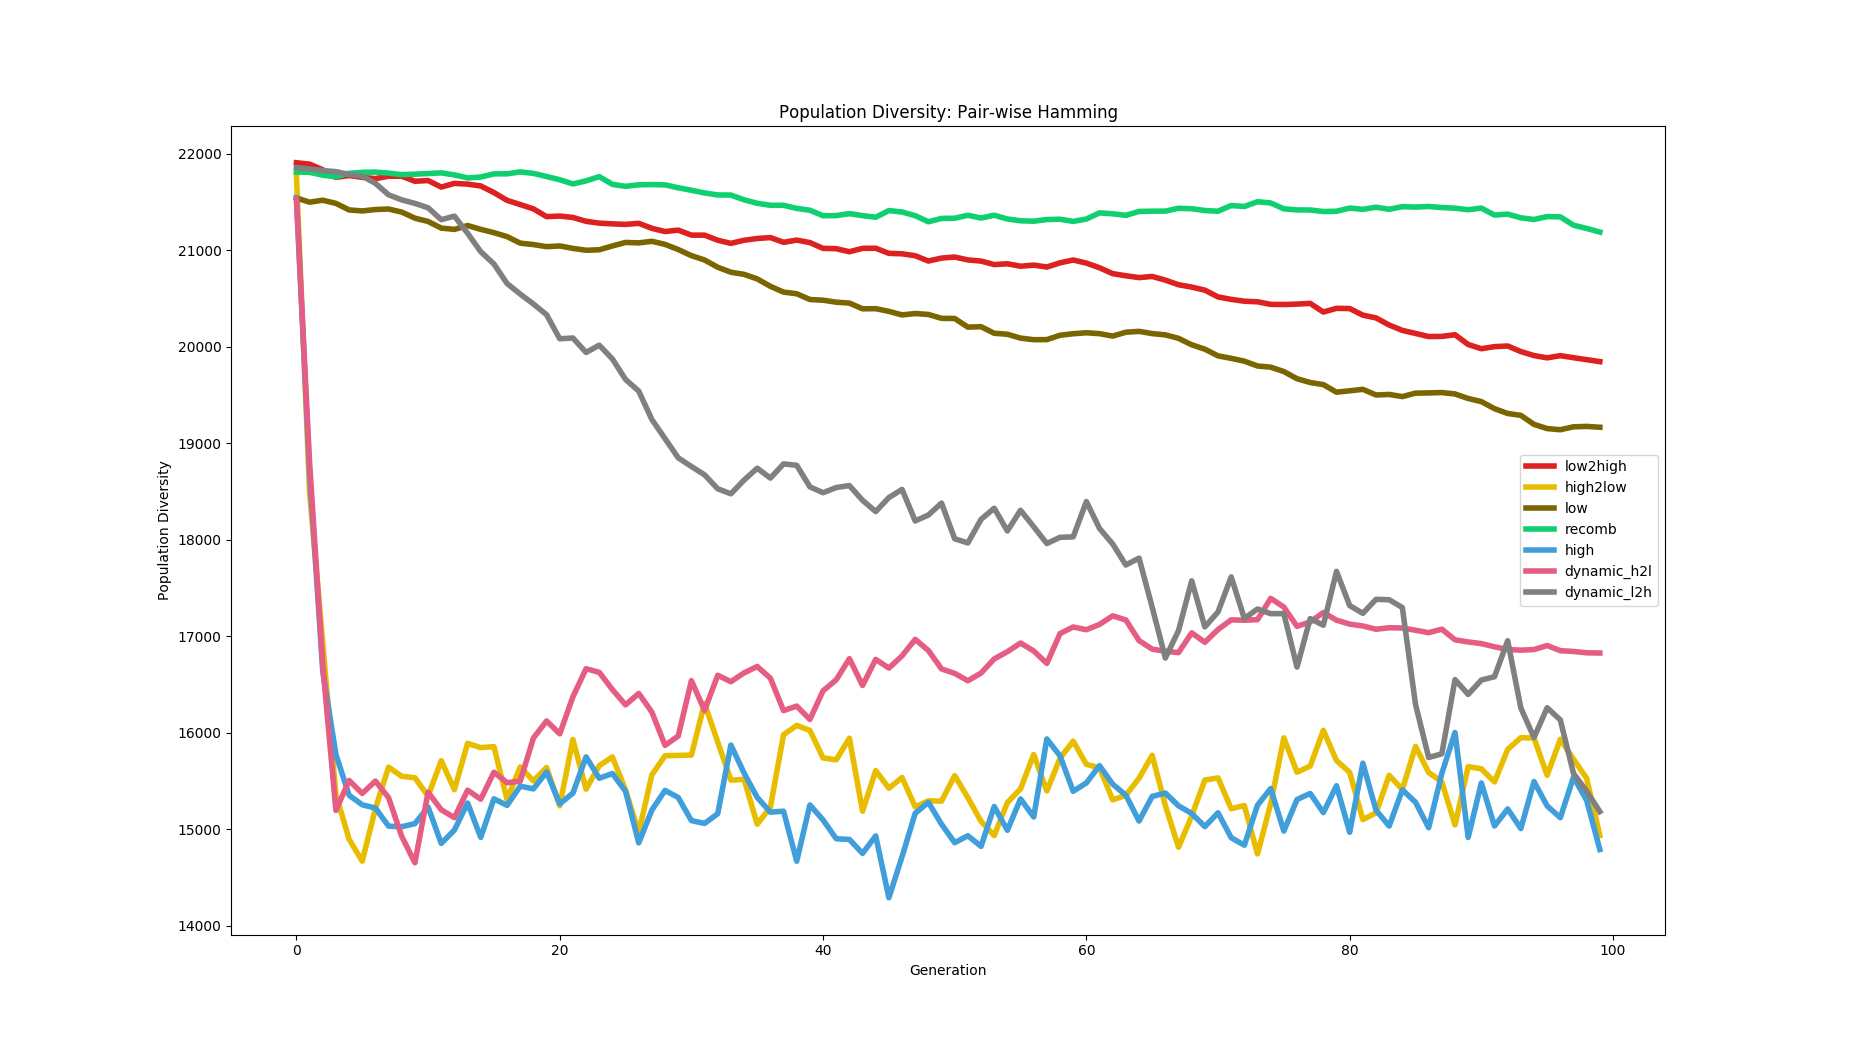
\includegraphics[width=\linewidth]{Chapters/Experiments/search_algo/figures/diversity_showcase_hamming.png}
        \caption{Pair-wise Hamming distance.}
    \end{subfigure}
    \hfill
    \begin{subfigure}[h]{0.49\linewidth}
        \label{fig:diversity_comparison:homemade}
        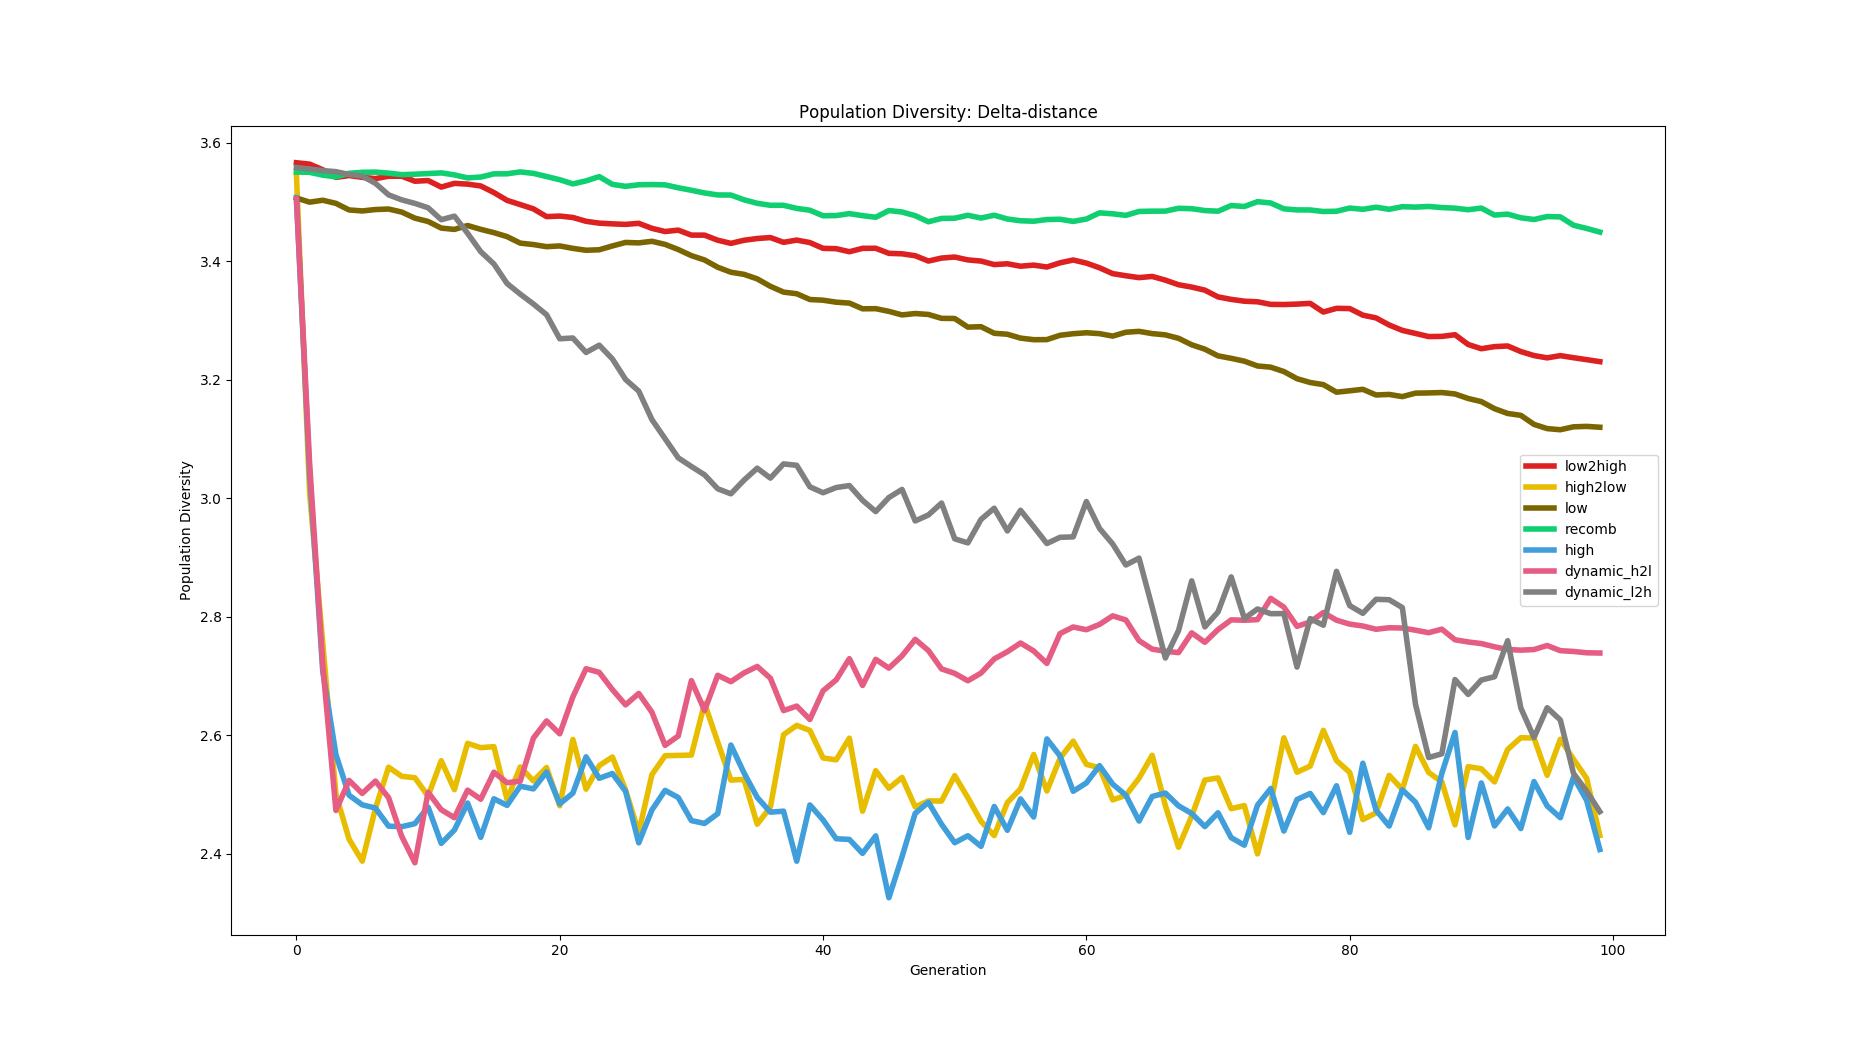
\includegraphics[width=\linewidth]{Chapters/Experiments/search_algo/figures/diversity_showcase_homemade.png}
        \caption{\(\Delta\)-diversity metric}
    \end{subfigure}%
    \caption{A comparison of pair-wise Hamming distance and \(\Delta\)-diversity. The diversity is the average population diversity for each generation during the search for an optimal path for task 1a. Note the similar curves for each algorithm and the scale on the y-axis}
\end{figure}
